\scanpage{5}
\mspage{1}

\uline{Courbes \inserted{exceptionnelles} de type} $(1,1)$ (sur $\mathbb C$)

A) \uline{Courbe \inserted{ell.} anharmonique de type carré}

Cat. de ces courbes \unsure{équivalente} : celle des carrés
\deleted{\unsure{équilatères}} orientés, i.e. des torseurs sur
\[
\mathbb Z/4\mathbb Z\simeq\mu_4(\mathbb C)\simeq
\text{groupe des unités algébriques de }\mathbb Q[i]
\]
\margin{i.e. groupe des unités de $\mathbb Z[i]$
\unsure{anneau} des entiers de $\mathbb Q[i]$}

La donnée d'un tel torseur \inserted{($S$)} permet de tordre
$\mathbb E\ell_0\overset{\mathrm{def}}\simeq
\mathbb C/\mathbb Z[i]$ et trouver
\[
\mathbb E\ell_0(S)\simeq\mathbb E\ell_0
\mathbin{\wedge}_{\mathbb Z/4\mathbb Z}S
\]

\margin{
\figure{
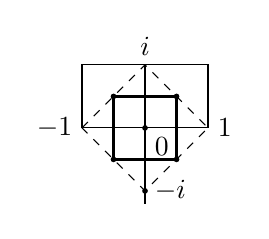
\begin{tikzpicture}[scale=.8]
\draw[thin] (-1,0)--(-1,1)--(1,1)--(1,0);
\draw[dashed] (-1,0)--(0,1)--(1,0)--(0,-1)--cycle;
\draw (-1,0)--(1,0);
\draw (0,-1.2)--(0,1);
\draw[thick] (-.5,-.5)--(-.5,.5)--(.5,.5)--(.5,-.5)--cycle;
\foreach \x/\y in {0/0,-.5/.5,.5/.5,.5/-.5,-.5/-.5,0/-1}
{\fill (\x,\y) circle (.045);}
\node[left] at (-1,0) {$-1$}; \node[right] at (1,0) {$1$};
\node[above] at (0,1) {$i$}; \node[right] at (0,-1) {$-i$};
\node[below right] at (0,0) {$0$};
\end{tikzpicture}
}}

Si le carré est réalisé comme un carré \inserted{au dedans}
dans un plan euclidien \inserted{$V_S$} (canoniquement), de centre $0$,
\deleted{
\figure{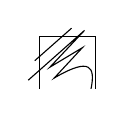
\begin{tikzpicture}[scale=.55]
\draw (0,0)--(0,1.2)--(1.3,1.2)--(1.3,0);
\draw (-.25,.2)--(1.05,1.35)--(.25,.5)--(1,.95)--(.35,.25)
 .. controls (1.2,.75) and (1.3,.5) .. (1.2,0);
\draw (-.1,.65)--(.75,1.4);
\end{tikzpicture}}
}
\figure{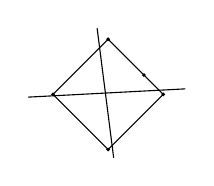
\begin{tikzpicture}[scale=.7]
\draw (-1,0)--(0,1)--(1,0)--(0,-1)--cycle;
\draw (-1.45,-.05)--(1.4,.1); \draw (.1,-1.15)--(-.2,1.2);
\foreach \x/\y in {-1/0,0/1,1/0,0/-1,.65/.35}
{\fill (\x,\y) circle (.035);}
\end{tikzpicture}}
on en déduit dans le plan (vectoriel via $0$) $V_S$
un syst. de deux \deleted{axes de}
coordonnées \inserted{mod. signes}
via les diagonales, d'où un
\deleted{\unsure{lattice}} \inserted{réseau}
$\Gamma_S$ dans $V_S$ (sous-groupe discret de
rang $2$) et
\[
\boxed{\mathbb E\ell_0(\unsure{S})\unsure{\simeq|/2}
X_S=V_S/\Gamma_S}.
\]

\margin{
\figure{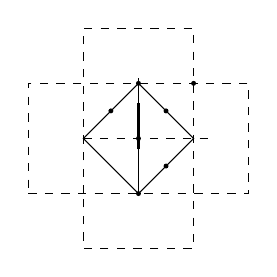
\begin{tikzpicture}[scale=.7]
\draw[dashed] (-1,-1)--(-1,2)--(1,2)--(1,-2)--(-1,-2)--(-1,-1);
\draw[dashed] (-2,-1)--(2,-1)--(2,1)--(-2,1)--cycle;
\draw (-1,0)--(0,1)--(1,0)--(0,-1)--cycle;
\draw[dashed] (-1,0)--(1.4,0);
\draw (0,-1)--(0,1.1);
\draw[very thick] (0,-.2)--(0,.65);
\foreach \x/\y in {0/0,0/1,0/-1,-.5/.5,.5/.5,.5/-.5,1/1}
{\fill (\x,\y) circle (.045);}
\end{tikzpicture}}
}

Il y a dans $X_S$ un élément d'ordre $2$ canonique
\inserted{$\unsure{\eta_S}$}
(stable par automorphismes), les deux autres él. d'
ordre $2$ sont échangés par le générateur $i$ de
$\mu_4(\mathbb C)\simeq\operatorname{Aut}(\unsure{X_S})$.
(\uline{NB} $\unsure{\eta_S}$ peut donc être défini

\margin{4}
